
%% bare_conf.tex
%% V1.3
%% 2007/01/11
%% by Michael Shell
%% See:
%% http://www.michaelshell.org/
%% for current contact information.
%%
%% This is a skeleton file demonstrating the use of IEEEtran.cls
%% (requires IEEEtran.cls version 1.7 or later) with an IEEE conference paper.
%%
%% Support sites:
%% http://www.michaelshell.org/tex/ieeetran/
%% http://www.ctan.org/tex-archive/macros/latex/contrib/IEEEtran/
%% and
%% http://www.ieee.org/

%%*************************************************************************
%% Legal Notice:
%% This code is offered as-is without any warranty either expressed or
%% implied; without even the implied warranty of MERCHANTABILITY or
%% FITNESS FOR A PARTICULAR PURPOSE! 
%% User assumes all risk.
%% In no event shall IEEE or any contributor to this code be liable for
%% any damages or losses, including, but not limited to, incidental,
%% consequential, or any other damages, resulting from the use or misuse
%% of any information contained here.
%%
%% All comments are the opinions of their respective authors and are not
%% necessarily endorsed by the IEEE.
%%
%% This work is distributed under the LaTeX Project Public License (LPPL)
%% ( http://www.latex-project.org/ ) version 1.3, and may be freely used,
%% distributed and modified. A copy of the LPPL, version 1.3, is included
%% in the base LaTeX documentation of all distributions of LaTeX released
%% 2003/12/01 or later.
%% Retain all contribution notices and credits.
%% ** Modified files should be clearly indicated as such, including  **
%% ** renaming them and changing author support contact information. **
%%
%% File list of work: IEEEtran.cls, IEEEtran_HOWTO.pdf, bare_adv.tex,
%%                    bare_conf.tex, bare_jrnl.tex, bare_jrnl_compsoc.tex
%%*************************************************************************

% *** Authors should verify (and, if needed, correct) their LaTeX system  ***
% *** with the testflow diagnostic prior to trusting their LaTeX platform ***
% *** with production work. IEEE's font choices can trigger bugs that do  ***
% *** not appear when using other class files.                            ***
% The testflow support page is at:
% http://www.michaelshell.org/tex/testflow/



% Note that the a4paper option is mainly intended so that authors in
% countries using A4 can easily print to A4 and see how their papers will
% look in print - the typesetting of the document will not typically be
% affected with changes in paper size (but the bottom and side margins will).
% Use the testflow package mentioned above to verify correct handling of
% both paper sizes by the user's LaTeX system.
%
% Also note that the "draftcls" or "draftclsnofoot", not "draft", option
% should be used if it is desired that the figures are to be displayed in
% draft mode.
%
\documentclass[10pt, conference, compsocconf]{IEEEtran}
% Add the compsocconf option for Computer Society conferences.
%
% If IEEEtran.cls has not been installed into the LaTeX system files,
% manually specify the path to it like:
% \documentclass[conference]{../sty/IEEEtran}





% Some very useful LaTeX packages include:
% (uncomment the ones you want to load)


% *** MISC UTILITY PACKAGES ***
%
%\usepackage{ifpdf}
% Heiko Oberdiek's ifpdf.sty is very useful if you need conditional
% compilation based on whether the output is pdf or dvi.
% usage:
% \ifpdf
%   % pdf code
% \else
%   % dvi code
% \fi
% The latest version of ifpdf.sty can be obtained from:
% http://www.ctan.org/tex-archive/macros/latex/contrib/oberdiek/
% Also, note that IEEEtran.cls V1.7 and later provides a builtin
% \ifCLASSINFOpdf conditional that works the same way.
% When switching from latex to pdflatex and vice-versa, the compiler may
% have to be run twice to clear warning/error messages.






% *** CITATION PACKAGES ***
%
%\usepackage{cite}
% cite.sty was written by Donald Arseneau
% V1.6 and later of IEEEtran pre-defines the format of the cite.sty package
% \cite{} output to follow that of IEEE. Loading the cite package will
% result in citation numbers being automatically sorted and properly
% "compressed/ranged". e.g., [1], [9], [2], [7], [5], [6] without using
% cite.sty will become [1], [2], [5]--[7], [9] using cite.sty. cite.sty's
% \cite will automatically add leading space, if needed. Use cite.sty's
% noadjust option (cite.sty V3.8 and later) if you want to turn this off.
% cite.sty is already installed on most LaTeX systems. Be sure and use
% version 4.0 (2003-05-27) and later if using hyperref.sty. cite.sty does
% not currently provide for hyperlinked citations.
% The latest version can be obtained at:
% http://www.ctan.org/tex-archive/macros/latex/contrib/cite/
% The documentation is contained in the cite.sty file itself.






% *** GRAPHICS RELATED PACKAGES ***
%
\ifCLASSINFOpdf
  \usepackage[pdftex]{graphicx}
  % declare the path(s) where your graphic files are
  \graphicspath{{./img/}}
  % and their extensions so you won't have to specify these with
  % every instance of \includegraphics
  % \DeclareGraphicsExtensions{.pdf,.jpeg,.png}
\else
  % or other class option (dvipsone, dvipdf, if not using dvips). graphicx
  % will default to the driver specified in the system graphics.cfg if no
  % driver is specified.
  \usepackage[dvips]{graphicx}
  % declare the path(s) where your graphic files are
  \graphicspath{{./img/}}
  % and their extensions so you won't have to specify these with
  % every instance of \includegraphics
  % \DeclareGraphicsExtensions{.eps}
\fi
% graphicx was written by David Carlisle and Sebastian Rahtz. It is
% required if you want graphics, photos, etc. graphicx.sty is already
% installed on most LaTeX systems. The latest version and documentation can
% be obtained at: 
% http://www.ctan.org/tex-archive/macros/latex/required/graphics/
% Another good source of documentation is "Using Imported Graphics in
% LaTeX2e" by Keith Reckdahl which can be found as epslatex.ps or
% epslatex.pdf at: http://www.ctan.org/tex-archive/info/
%
% latex, and pdflatex in dvi mode, support graphics in encapsulated
% postscript (.eps) format. pdflatex in pdf mode supports graphics
% in .pdf, .jpeg, .png and .mps (metapost) formats. Users should ensure
% that all non-photo figures use a vector format (.eps, .pdf, .mps) and
% not a bitmapped formats (.jpeg, .png). IEEE frowns on bitmapped formats
% which can result in "jaggedy"/blurry rendering of lines and letters as
% well as large increases in file sizes.
%
% You can find documentation about the pdfTeX application at:
% http://www.tug.org/applications/pdftex





% *** MATH PACKAGES ***
%
\usepackage{amssymb}
%\usepackage[cmex10]{amsmath}
% A popular package from the American Mathematical Society that provides
% many useful and powerful commands for dealing with mathematics. If using
% it, be sure to load this package with the cmex10 option to ensure that
% only type 1 fonts will utilized at all point sizes. Without this option,
% it is possible that some math symbols, particularly those within
% footnotes, will be rendered in bitmap form which will result in a
% document that can not be IEEE Xplore compliant!
%
% Also, note that the amsmath package sets \interdisplaylinepenalty to 10000
% thus preventing page breaks from occurring within multiline equations. Use:
%\interdisplaylinepenalty=2500
% after loading amsmath to restore such page breaks as IEEEtran.cls normally
% does. amsmath.sty is already installed on most LaTeX systems. The latest
% version and documentation can be obtained at:
% http://www.ctan.org/tex-archive/macros/latex/required/amslatex/math/





% *** SPECIALIZED LIST PACKAGES ***
%
%\usepackage{algorithmic}
% algorithmic.sty was written by Peter Williams and Rogerio Brito.
% This package provides an algorithmic environment fo describing algorithms.
% You can use the algorithmic environment in-text or within a figure
% environment to provide for a floating algorithm. Do NOT use the algorithm
% floating environment provided by algorithm.sty (by the same authors) or
% algorithm2e.sty (by Christophe Fiorio) as IEEE does not use dedicated
% algorithm float types and packages that provide these will not provide
% correct IEEE style captions. The latest version and documentation of
% algorithmic.sty can be obtained at:
% http://www.ctan.org/tex-archive/macros/latex/contrib/algorithms/
% There is also a support site at:
% http://algorithms.berlios.de/index.html
% Also of interest may be the (relatively newer and more customizable)
% algorithmicx.sty package by Szasz Janos:
% http://www.ctan.org/tex-archive/macros/latex/contrib/algorithmicx/




% *** ALIGNMENT PACKAGES ***
%
%\usepackage{array}
% Frank Mittelbach's and David Carlisle's array.sty patches and improves
% the standard LaTeX2e array and tabular environments to provide better
% appearance and additional user controls. As the default LaTeX2e table
% generation code is lacking to the point of almost being broken with
% respect to the quality of the end results, all users are strongly
% advised to use an enhanced (at the very least that provided by array.sty)
% set of table tools. array.sty is already installed on most systems. The
% latest version and documentation can be obtained at:
% http://www.ctan.org/tex-archive/macros/latex/required/tools/


%\usepackage{mdwmath}
%\usepackage{mdwtab}
% Also highly recommended is Mark Wooding's extremely powerful MDW tools,
% especially mdwmath.sty and mdwtab.sty which are used to format equations
% and tables, respectively. The MDWtools set is already installed on most
% LaTeX systems. The lastest version and documentation is available at:
% http://www.ctan.org/tex-archive/macros/latex/contrib/mdwtools/


% IEEEtran contains the IEEEeqnarray family of commands that can be used to
% generate multiline equations as well as matrices, tables, etc., of high
% quality.


%\usepackage{eqparbox}
% Also of notable interest is Scott Pakin's eqparbox package for creating
% (automatically sized) equal width boxes - aka "natural width parboxes".
% Available at:
% http://www.ctan.org/tex-archive/macros/latex/contrib/eqparbox/





% *** SUBFIGURE PACKAGES ***
%\usepackage[tight,footnotesize]{subfigure}
% subfigure.sty was written by Steven Douglas Cochran. This package makes it
% easy to put subfigures in your figures. e.g., "Figure 1a and 1b". For IEEE
% work, it is a good idea to load it with the tight package option to reduce
% the amount of white space around the subfigures. subfigure.sty is already
% installed on most LaTeX systems. The latest version and documentation can
% be obtained at:
% http://www.ctan.org/tex-archive/obsolete/macros/latex/contrib/subfigure/
% subfigure.sty has been superceeded by subfig.sty.



%\usepackage[caption=false]{caption}
%\usepackage[font=footnotesize]{subfig}
% subfig.sty, also written by Steven Douglas Cochran, is the modern
% replacement for subfigure.sty. However, subfig.sty requires and
% automatically loads Axel Sommerfeldt's caption.sty which will override
% IEEEtran.cls handling of captions and this will result in nonIEEE style
% figure/table captions. To prevent this problem, be sure and preload
% caption.sty with its "caption=false" package option. This is will preserve
% IEEEtran.cls handing of captions. Version 1.3 (2005/06/28) and later 
% (recommended due to many improvements over 1.2) of subfig.sty supports
% the caption=false option directly:
%\usepackage[caption=false,font=footnotesize]{subfig}
%
% The latest version and documentation can be obtained at:
% http://www.ctan.org/tex-archive/macros/latex/contrib/subfig/
% The latest version and documentation of caption.sty can be obtained at:
% http://www.ctan.org/tex-archive/macros/latex/contrib/caption/




% *** FLOAT PACKAGES ***
%
%\usepackage{fixltx2e}
% fixltx2e, the successor to the earlier fix2col.sty, was written by
% Frank Mittelbach and David Carlisle. This package corrects a few problems
% in the LaTeX2e kernel, the most notable of which is that in current
% LaTeX2e releases, the ordering of single and double column floats is not
% guaranteed to be preserved. Thus, an unpatched LaTeX2e can allow a
% single column figure to be placed prior to an earlier double column
% figure. The latest version and documentation can be found at:
% http://www.ctan.org/tex-archive/macros/latex/base/



%\usepackage{stfloats}
% stfloats.sty was written by Sigitas Tolusis. This package gives LaTeX2e
% the ability to do double column floats at the bottom of the page as well
% as the top. (e.g., "\begin{figure*}[!b]" is not normally possible in
% LaTeX2e). It also provides a command:
%\fnbelowfloat
% to enable the placement of footnotes below bottom floats (the standard
% LaTeX2e kernel puts them above bottom floats). This is an invasive package
% which rewrites many portions of the LaTeX2e float routines. It may not work
% with other packages that modify the LaTeX2e float routines. The latest
% version and documentation can be obtained at:
% http://www.ctan.org/tex-archive/macros/latex/contrib/sttools/
% Documentation is contained in the stfloats.sty comments as well as in the
% presfull.pdf file. Do not use the stfloats baselinefloat ability as IEEE
% does not allow \baselineskip to stretch. Authors submitting work to the
% IEEE should note that IEEE rarely uses double column equations and
% that authors should try to avoid such use. Do not be tempted to use the
% cuted.sty or midfloat.sty packages (also by Sigitas Tolusis) as IEEE does
% not format its papers in such ways.





% *** PDF, URL AND HYPERLINK PACKAGES ***
%
\usepackage{url}
% url.sty was written by Donald Arseneau. It provides better support for
% handling and breaking URLs. url.sty is already installed on most LaTeX
% systems. The latest version can be obtained at:
% http://www.ctan.org/tex-archive/macros/latex/contrib/misc/
% Read the url.sty source comments for usage information. Basically,
% \url{my_url_here}.





% *** Do not adjust lengths that control margins, column widths, etc. ***
% *** Do not use packages that alter fonts (such as pslatex).         ***
% There should be no need to do such things with IEEEtran.cls V1.6 and later.
% (Unless specifically asked to do so by the journal or conference you plan
% to submit to, of course. )


% correct bad hyphenation here
\hyphenation{op-tical net-works semi-conduc-tor}


\begin{document}
%
% paper title
% can use linebreaks \\ within to get better formatting as desired
\title{Semantic Annotation Semantically:\\Using a~Shareable Extraction Ontology and a Reasoner}


% author names and affiliations
% use a multiple column layout for up to two different
% affiliations

\author{\IEEEauthorblockN{Jan D\v{e}dek}
\IEEEauthorblockA{Department of Software Engineering\\
Charles University\\
Prague, Czech Republic\\
\url{dedek@ksi.mff.cuni.cz}}
\and
\IEEEauthorblockN{Peter Vojt\'{a}\v{s}}
\IEEEauthorblockA{Department of Software Engineering\\
Charles University\\
Prague, Czech Republic\\
\url{vojtas@ksi.mff.cuni.cz}}
}

% conference papers do not typically use \thanks and this command
% is locked out in conference mode. If really needed, such as for
% the acknowledgment of grants, issue a \IEEEoverridecommandlockouts
% after \documentclass

% for over three affiliations, or if they all won't fit within the width
% of the page, use this alternative format:
% 
%\author{\IEEEauthorblockN{Michael Shell\IEEEauthorrefmark{1},
%Homer Simpson\IEEEauthorrefmark{2},
%James Kirk\IEEEauthorrefmark{3}, 
%Montgomery Scott\IEEEauthorrefmark{3} and
%Eldon Tyrell\IEEEauthorrefmark{4}}
%\IEEEauthorblockA{\IEEEauthorrefmark{1}School of Electrical and Computer Engineering\\
%Georgia Institute of Technology,
%Atlanta, Georgia 30332--0250\\ Email: see http://www.michaelshell.org/contact.html}
%\IEEEauthorblockA{\IEEEauthorrefmark{2}Twentieth Century Fox, Springfield, USA\\
%Email: homer@thesimpsons.com}
%\IEEEauthorblockA{\IEEEauthorrefmark{3}Starfleet Academy, San Francisco, California 96678-2391\\
%Telephone: (800) 555--1212, Fax: (888) 555--1212}
%\IEEEauthorblockA{\IEEEauthorrefmark{4}Tyrell Inc., 123 Replicant Street, Los Angeles, California 90210--4321}}




% use for special paper notices
%\IEEEspecialpapernotice{(Invited Paper)}




% make the title area
\maketitle


\begin{abstract}
Information extraction (IE) and automated semantic annotation of text are usually done by complex tools. These tools use some kind of a model that represents the actual task and its solution. The model is usually represented as a set of extraction rules (e.g. regular expressions), gazetteer lists, or it is based on some statistical measurements and probability assertions. In the environment of the Semantic Web it is essential that information is shareable and some ontology based IE tools keep the model in so called extraction ontologies. In practice the extraction ontologies are usually strongly dependent on a particular extraction/annotation tool and cannot be used separately. In this paper we present an extension of the idea of extraction ontologies. 
According to the presented concept the extraction ontologies should not be dependent on the particular extraction/annotation tool. In our solution the extraction/annotation process can be done separately by an ordinary reasoner. 

We also present a proof of a concept for the idea: a case study with a linguistically based IE engine that exports its extraction rules to an extraction ontology and we demonstrate how this extraction ontology can be applied to a document by a reasoner. The paper also contains an evaluation experiment with several OWL reasoners.
\end{abstract}

\begin{IEEEkeywords}
Extraction Ontology; Reasoning; Information Extraction; Semantic Annotation
\end{IEEEkeywords}


% For peer review papers, you can put extra information on the cover
% page as needed:
% \ifCLASSOPTIONpeerreview
% \begin{center} \bfseries EDICS Category: 3-BBND \end{center}
% \fi
%
% For peerreview papers, this IEEEtran command inserts a page break and
% creates the second title. It will be ignored for other modes.
\IEEEpeerreviewmaketitle



%%%%%%%%%%%%%%%%%%%%%%%%%%%%%%%%%%%%%%%%%%%%%%%%%%%%%%%%%%%%%%%%%%%%%%%%%%%%%%%%%%%%%%%%%%%%%%%%%%%%%%%%%%%%%%
\section{Introduction}
%%%%%%%%%%%%%%%%%%%%%%%%%%%%%%%%%%%%%%%%%%%%%%%%%%%%%%%%%%%%%%%%%%%%%%%%%%%%%%%%%%%%%%%%%%%%%%%%%%%%%%%%%%%%%%


Information extraction (IE) and automated semantic annotation of text are usually done by complex tools and all these tools use some kind of a model that represents the actual task and its solution. The model is usually represented as a set of some kind of extraction rules (e.g. regular expressions), gazetteer lists or it is based on some statistical measurements and probability assertions (classification algorithms like Support Vector Machines (SVM), Maximum Entropy Models, Decision Trees, Hidden Markov Models (HMM), Conditional Random Fields (CRF), etc.)

In the beginning a model is either created by a human user or it is learned from a training dataset. Then, in an actual extraction/annotation process, the model is used as a configuration or as an input parameter of the particular extraction/annotation tool. These models are usually stored in proprietary formats and they are accessible only by the corresponding tool.

In the environment of the Semantic Web it is essential that information is shareable and some ontology based IE tools keep the model in so called extraction ontologies. Extraction ontologies should serve as a wrapper for documents of a narrow domain of interest. When we apply an extraction ontology to a document, the ontology identifies objects and relationships present in the document and it associates them with the corresponding ontology terms and thus wraps the document so that it is understandable in terms of the ontology \cite{DBLP:conf/er/EmbleyTL02}.



In practice the extraction ontologies are usually strongly dependent on a particular extraction/annotation tool and cannot be used separately. The strong dependency of an extraction ontology on the corresponding tool makes it very difficult to share. When an extraction ontology cannot be used outside the tool there is also no need to keep the ontology in a standard ontology format such as RDF\footnote{\url{http://www.w3.org/RDF/}} or OWL\footnote{\url{http://www.w3.org/2001/sw/wiki/OWL}}. The only way how to use such extraction ontology is within the corresponding extraction tool. It is not necessary to have the ontology in a `owl' or `rdf' file. In a sense such extraction ontology is just a configuration file. For example in \cite{springerlink:10.1007/978-3-642-01891-6_5} %[Labsky]
 (and also in \cite{DBLP:conf/er/EmbleyTL02}) the so called extraction ontologies are kept in XML files with a proprietary structure and it is absolutely sufficient, there is no need to treat them differently.



\subsection{Shareable Extraction Ontologies}

In this paper we present an extension of the idea of extraction ontologies. We adopt the point that extraction models are kept in extraction ontologies and we add that the extraction ontologies should not be dependent on the particular extraction/annotation tool. In such case the extraction/annotation process can be done separately by an ordinary reasoner.


In this paper we present a proof of a concept for the idea: a case study with our linguistically based IE engine and an experiment with several OWL reasoners. In the case study (see Section~\ref{sec:case}) the IE engine exports its extraction rules to the form of an extraction ontology. Third party linguistic tool linguistically annotates an input document and the linguistic annotations are translated to so-called document ontology. After that an ordinary OWL reasoner is used to apply the extraction ontology on the document ontology, which has the same effect as a direct application of the extraction rules on the document.
In Section~\ref{sec:experiment} we present an experiment with several OWL reasoner and IE datasets to verify feasibility of the idea.  




%%%%%%%%%%%%%%%%%%%%%%%%%%%%%%%%%%%%%%%%%%%%%%%%%%%%%%%%%%%%%%%%%%%%%%%%%%%%%%%%%%%%%%%%%%%%%%%%%%%%%%%%%%%%%%
\section{Related Work}
%%%%%%%%%%%%%%%%%%%%%%%%%%%%%%%%%%%%%%%%%%%%%%%%%%%%%%%%%%%%%%%%%%%%%%%%%%%%%%%%%%%%%%%%%%%%%%%%%%%%%%%%%%%%%%
Ontology-based Information Extraction (OBIE) \cite{citeulike:7291004} or Ontology-driven Information Extraction \cite{Yildiz:2007:OMO:1793154.1793216} has recently emerged as a subfield of information extraction. Furthermore, Web Information Extraction \cite{DBLP:journals/tkde/ChangKGS06} is a closely related discipline. Many extraction and annotation tools can be found in the above mentioned surveys \cite{citeulike:7291004,DBLP:journals/tkde/ChangKGS06} and many of the tools also use an ontology as an output format, but almost all of them store their extraction models in proprietary formats and the models are accessible only by the corresponding tool.

In the literature we have found only two approaches that use extraction ontologies. The former one was published by D. Embley \cite{DBLP:conf/er/EmbleyTL02,Embley:2004:TSU:1012294.1012295}
and the later one -- IE system Ex\footnote{\url{http://eso.vse.cz/~labsky/ex/}} was developped by M. Labsk\'{y} \cite{springerlink:10.1007/978-3-642-01891-6_5}. 
But in both cases the extraction ontologies are dependent on the particular tool and they are kept in XML files with a proprietary structure.


Also authors of \cite{citeulike:7291004} (a recent survey of OBIE systems) do not agree with allowing for extraction rules to be a part of an ontology. They use two arguments against that:
\begin{enumerate}
	\item Extraction rules are known to contain errors (because they are never 100\% accurate), and objections can be raised on their inclusion in ontologies in terms of formality and accuracy.

	\item It is hard to argue that linguistic extraction rules should be considered a part of an ontology while information extractors based on other IE techniques (such as SVM, HMM, CRF, etc. classifiers used to identify instances of a class when classification is used as the IE technique) should be kept out of it: all IE techniques perform the same task with comparable effectiveness (generally successful but not 100\% accurate). But the techniques advocated for the inclusion of linguistic rules in ontologies cannot accommodate such IE techniques.
	
The authors then conclude that either all information extractors (that use different IE techniques) should be included in the ontologies or none should be included.
\end{enumerate}



Concerning the first argument, we have to take into account that extraction ontologies are not ordinary ontologies, it should be agreed that they do not contain 100\% accurate knowledge. Also the estimated accuracy of the extraction rules can be saved in the extraction ontology and it can then help potential users to decide how much they will trust the extraction ontology.

Concerning the second argument, we agree that it is not always possible to save an extraction model to an ontology. But on the other hand we think that there are cases when shareable extraction ontologies can be useful. And maybe in the future; if this idea proves its usefulness; new standard ways how to encode models to an ontology will appear.


Also the most widely agreed definitions of an ontology emphasize the shared aspect of ontologies: 
\begin{quote}
An ontology is a formal specification of a shared conceptualization.	\cite{so17864}
\end{quote}

\begin{quote}
An ontology is a formal, explicit specification of a shared conceptualization. \cite{Studer1998161}
\end{quote}

Of course the word `shareable' has different meaning from `shared'. Something that is shareable is not necessarily shared, but on the other hand something that is shared should be shareable. We do not think that shareable extraction ontologies will contain shared knowledge about how to extract data from documents in certain domain. This is for example not true for all extraction models artificially learned from a training corpus. Here shareable simply means that the extraction rules can be shared amongst software agents and can be used separately from the original tool. In time it will turn out if such extraction ontologies are useful or not. But for sure they bring something new that was not possible before.






%%%%%%%%%%%%%%%%%%%%%%%%%%%%%%%%%%%%%%%%%%%%%%%%%%%%%%%%%%%%%%%%%%%%%%%%%%%%%%%%%%%%%%%%%%%%%%%%%%%%%%%%%%%%%%
\section{The Main Idea Illustrated -- Our Case Study} \label{sec:case}
%%%%%%%%%%%%%%%%%%%%%%%%%%%%%%%%%%%%%%%%%%%%%%%%%%%%%%%%%%%%%%%%%%%%%%%%%%%%%%%%%%%%%%%%%%%%%%%%%%%%%%%%%%%%%%

In this section we will describe the main idea of the paper and we will illustrate it with a case study.

\subsection{Document Ontologies} \label{sec:doc_ont}

The main idea of this paper assumes that extraction ontologies will be shareable and they can be applied on a document outside of the original extraction/annotation tool. And we assert that the extraction ontologies can be applied by ordinary reasoners. This assumption implies that both extraction ontologies and documents have to be in a reasoner readable format. In the case of contemporary OWL reasoners there are standard reasoner-readable languages: OWL and RDF in a rich variety of possible serializations (XML, Turtle, N-Triples, etc.) Besides that there exists standard ways like GRDDL\footnote{\url{http://www.w3.org/TR/grddl/}} or RDFa\footnote{\url{http://www.w3.org/TR/xhtml-rdfa-primer/}} to transform an ordinary document to a RDF document. We call the output of such transformation a `document ontology'. A document ontology should contain all relevant data of a document and preferably the document could be reconstructed from the document ontology on demand.

When a reasoner is applying an extraction ontology to a document, it only has ``to annotate'' the corresponding document ontology, not the document itself. Here ``to annotate'' means to add new knowledge -- new class membership or property assertions. In fact it means just to do the inference tasks prescribed by the extraction ontology on the document ontology. 


\subsection{Implementation}

In this section we will present details about the case study.  We have used our IE engine \cite{biblio:DedekISWC2010} based on deep linguistic parsing and Inductive Logic Programming. It is a complex system implemented with a great help of the GATE system\footnote{\url{http://gate.ac.uk/}} \cite{dedek:GATE_ACL2002} and it also uses many other third party tools including several linguistic tools and a Prolog system. Installation and making the system operate is not simple. This case study should demonstrate that the extraction rules produced by the system are not dependent on the system in the sense described above.




\subsubsection{Linguistic Analysis}


\begin{figure}
\centerline{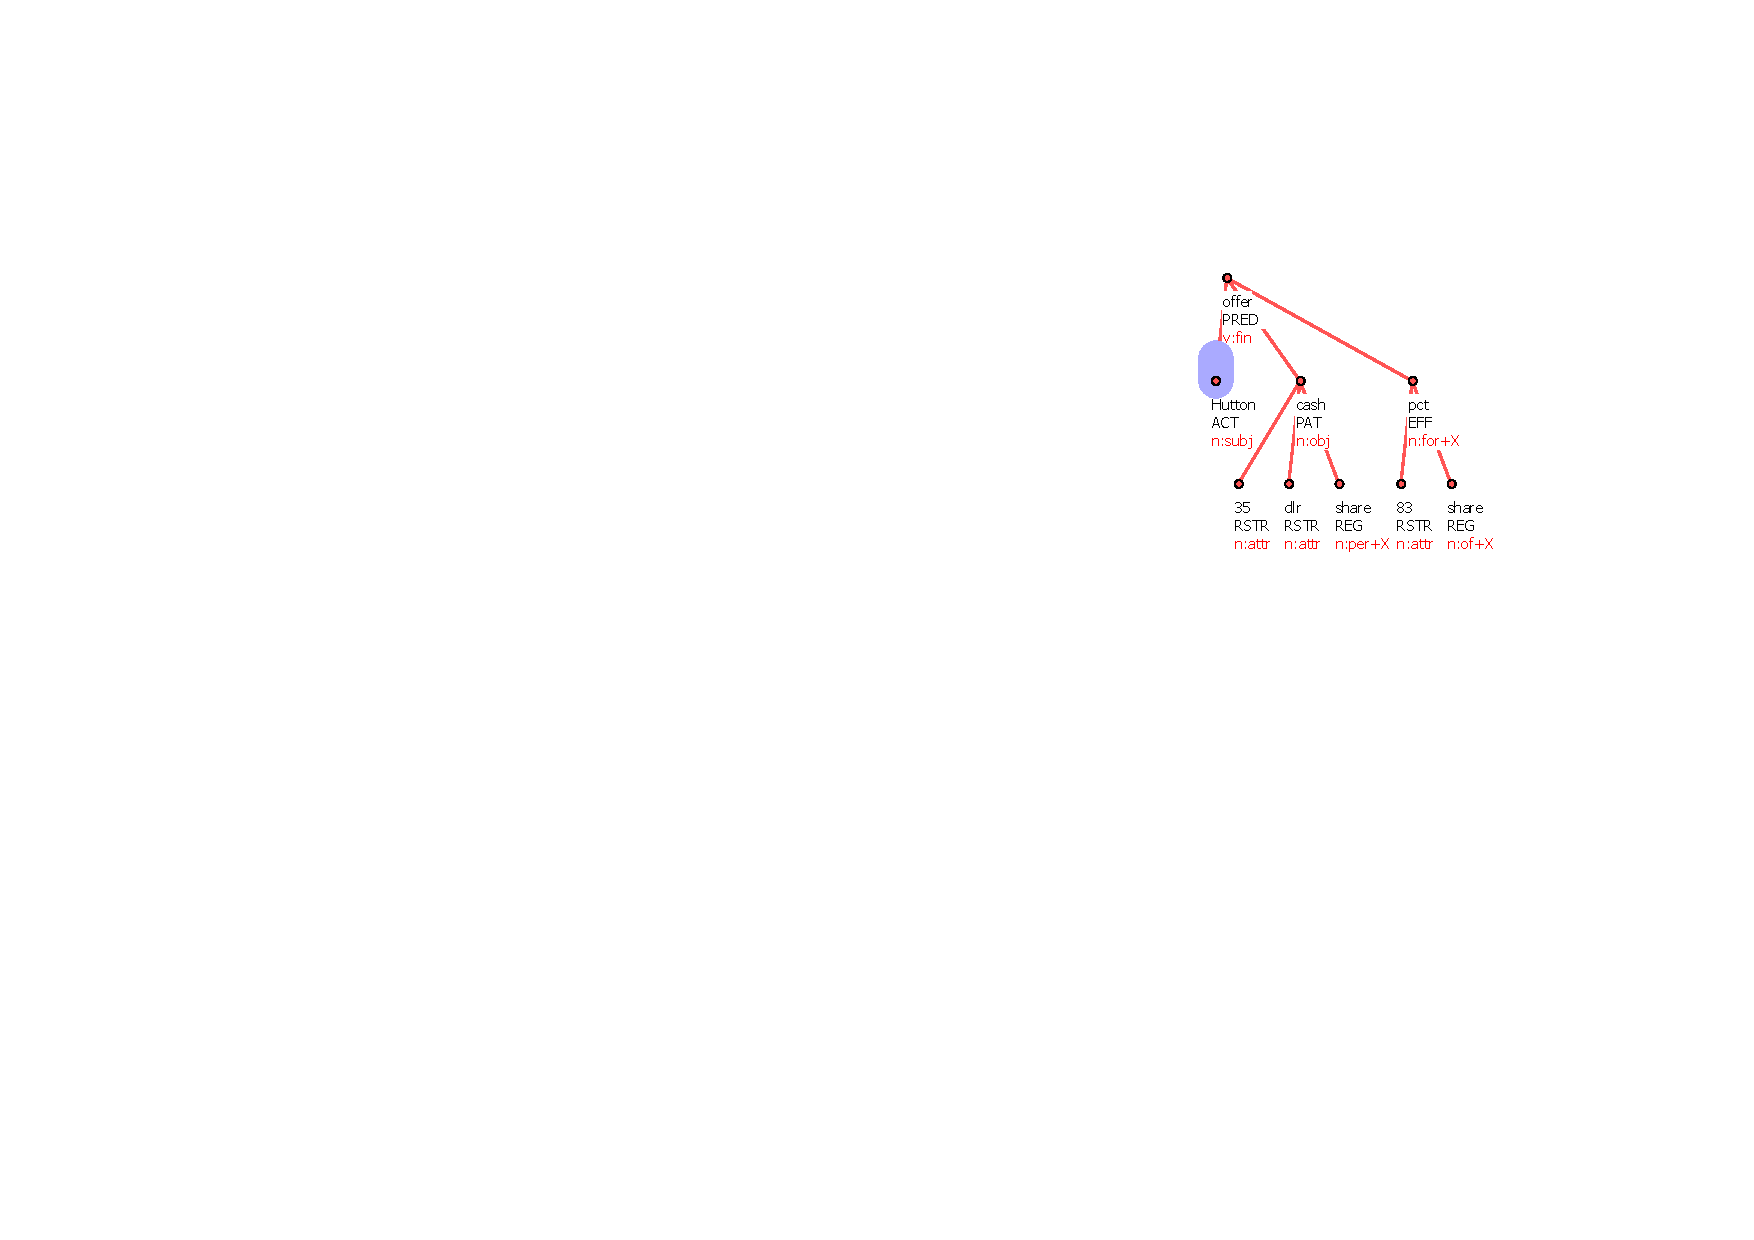
\includegraphics[width=0.7\hsize]{tree}}
\caption{Tectogrammatical tree of the sentence: ``Hutton is offering 35 dlrs cash per share for 83 pct of the shares.''
Nodes roughly correspond with words of a sentence, edges represent linguistic dependencies between nodes and some linguistic features (tectogrammatical lemma, semantic functor and semantic part of speech) are printed under each node. The node `Hutton' is decorated as a named entity.}
\label{img:tree}
\end{figure}


Our IE engine needs a linguistic preprocessing (deep linguistic parsing) of documents on its input. Deep linguistic parsing brings a very complex structure to the text and the structure serves as a footing for construction and application of extraction rules. 

We usually use TectoMT system\footnote{\url{http://ufal.mff.cuni.cz/tectomt/}} \cite{dedek:ZaPtTectoMTHighly2008} to do the linguistic preprocessing. TectoMT is a Czech project that contains many linguistic analyzers for different languages including Czech and English. We are using a majority of applicable tools from TectoMT: a tokeniser, a sentence splitter, morphological analyzers (including POS tagger), a syntactic parser and the deep syntactic (tectogrammatical) parser. All the tools are based on the dependency based linguistic theory and formalism of the Prague Dependency Treebank project\footnote{\url{http://ufal.mff.cuni.cz/pdt2.0/}} \cite{dedek:PDT20_CD}.

The output linguistic annotations of the TectoMT system are stored (along with the text of the source document) in XML files in so called Prague Markup Language\footnote{\url{http://ufal.mff.cuni.cz/jazz/PML/}} (PML). PML is a very complex language (or XML schema) that is able to express many linguistic elements and features present in text. For the IE engine a tree dependency structure of words in sentences is the most useful one because the edges of the structure guide the extraction rules. An example of such (tectogrammatical) tree structure is in Fig.~\ref{img:tree}.

In this case study PML files made from source documents by TectoMT are transformed to RDF document ontology by a quite simple GRDDL/XSLT\footnote{\url{http://www.w3.org/TR/xslt}} transformation. Such document ontology contains the whole variety of PML in RDF format.







\subsubsection{Rule Transformations}

Extraction rules produced by the IE engine are natively kept in a Prolog format; examples can be seen in Fig.~\ref{img:rules_prolog}. The engine is capable to export them to the OWL/XML\footnote{\url{http://www.w3.org/TR/owl-xmlsyntax/}} syntax for rules in OWL 2 \cite{GHPP09a} (see in Fig.~\ref{img:rules_xml}). Such rules can be parsed by OWL API\footnote{\url{http://owlapi.sourceforge.net/}} 3.1. Fig.~\ref{img:rules_protege} shows the example rules in Prot\'{e}g\'{e}\footnote{\url{http://protege.stanford.edu/}} 4 -- Rules View's format. And the last rule example can be seen in Fig.~\ref{img:rules_jena}, it shows a rule in the Jena rules format\footnote{\url{http://jena.sourceforge.net/inference/#RULEsyntax}}. Conversion to Jena rules was necessary because it is the only format that Jena can parse, see details about our use of Jena in Section~\ref{sec:experiment}. The Jena rules were obtained using following transformation process: OWL/XML $\rightarrow$ RDF/SWRL\footnote{\url{http://www.w3.org/Submission/SWRL/}} conversion using OWL API and RDF/SWRL $\rightarrow$ Jena rules conversion using SweetRules\footnote{\url{http://sweetrules.semwebcentral.org/}}.



\begin{figure}
\small
[Rule 1] [Pos cover = 23 Neg cover = 6]\\
\verb@mention_root(acquired,A) :-@\\
\verb@   'lex.rf'(B,A), t_lemma(B,'Inc'),@\\
\verb@   tDependency(C,B), tDependency(C,D),@\\
\verb@   formeme(D,'n:in+X'), tDependency(E,C).@
\smallskip\newline
[Rule 11] [Pos cover = 25 Neg cover = 6]\\
\verb@mention_root(acquired,A) :-@\\
\verb@   'lex.rf'(B,A), t_lemma(B,'Inc'),@\\
\verb@   tDependency(C,B), formeme(C,'n:obj'), @\\
\verb@   tDependency(C,D), functor(D,'APP').@
\smallskip\newline
[Rule 75] [Pos cover = 14 Neg cover = 1]\\
\verb@mention_root(acquired,A) :-@\\
\verb@   'lex.rf'(B,A), t_lemma(B,'Inc'),@\\
\verb@   functor(B,'APP'), tDependency(C,B), @\\
\verb@   number(C,pl).@
	\caption{Examples of extraction rules in the native Prolog format.}
	\label{img:rules_prolog}
\end{figure}

\begin{figure}
\small
[Rule 1]\\
\verb@lex.rf(?b, ?a), t_lemma(?b, "Inc"),@\\
\verb@tDependency(?c, ?b), tDependency(?c, ?d),@\\
\verb@formeme(?d, "n:in+X"), tDependency(?c, ?e)@\\
\verb@      -> mention_root(?a, "acquired")@
\smallskip\newline
[Rule 11]\\
\verb@lex.rf(?b, ?a), t_lemma(?b, "Inc"),@\\
\verb@tDependency(?c, ?b), formeme(?c, "n:obj"),@\\
\verb@tDependency(?c, ?d), functor(?d, "APP")@\\
\verb@      -> mention_root(?a, "acquired")@   
\smallskip\newline
[Rule 75]\\
\verb@lex.rf(?b, ?a), t_lemma(?b, "Inc"),@\\
\verb@functor(?b, "APP"), tDependency(?c, ?b),@\\
\verb@number(?c, "pl")@\\
\verb@      -> mention_root(?a, "acquired")@   
	\caption{Examples of extraction rules in Prot\'{e}g\'{e} 4 -- Rules View's format}
	\label{img:rules_protege}
\end{figure}

\begin{figure}
\centerline{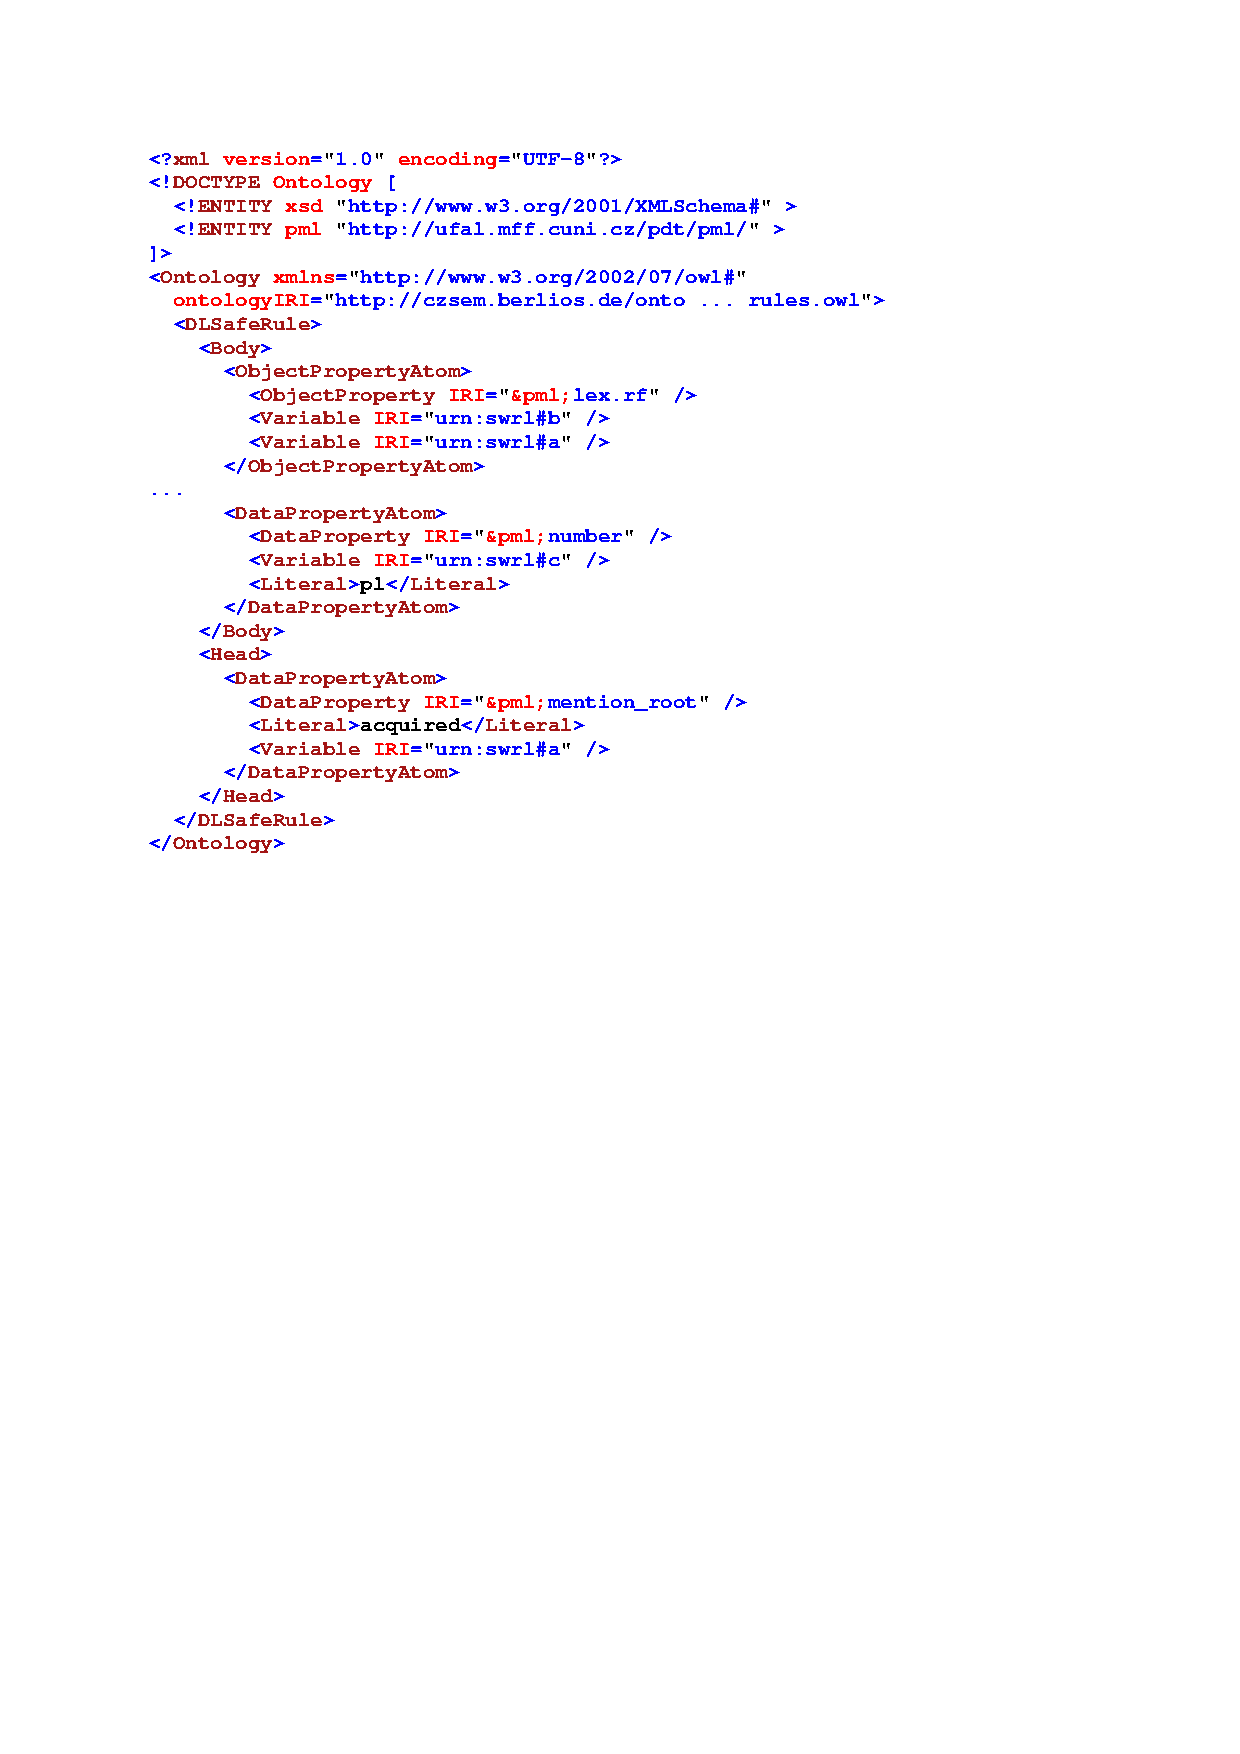
\includegraphics[width=\hsize]{rules_owl_xml}}
\caption{Rule 75 in the OWL/XML syntax for Rules in OWL 2 \cite{GHPP09a}.}
\label{img:rules_xml}
\end{figure}


\begin{figure}
\small
\begin{verbatim}
@prefix pml: <http://ufal.mff.cuni.cz/pdt/pml/>.
[rule-75:  
        ( ?b pml:lex.rf ?a )
        ( ?c pml:tDependency ?b )
        ( ?b pml:functor 'APP' )
        ( ?c pml:number 'pl' )
        ( ?b pml:t_lemma 'Inc' )
     -> 
        ( ?a pml:mention_root 'acquired' )
]
\end{verbatim}
\caption{Rule 75 in the Jena rules syntax.}
\label{img:rules_jena}
\end{figure}

\begin{figure*}
\centerline{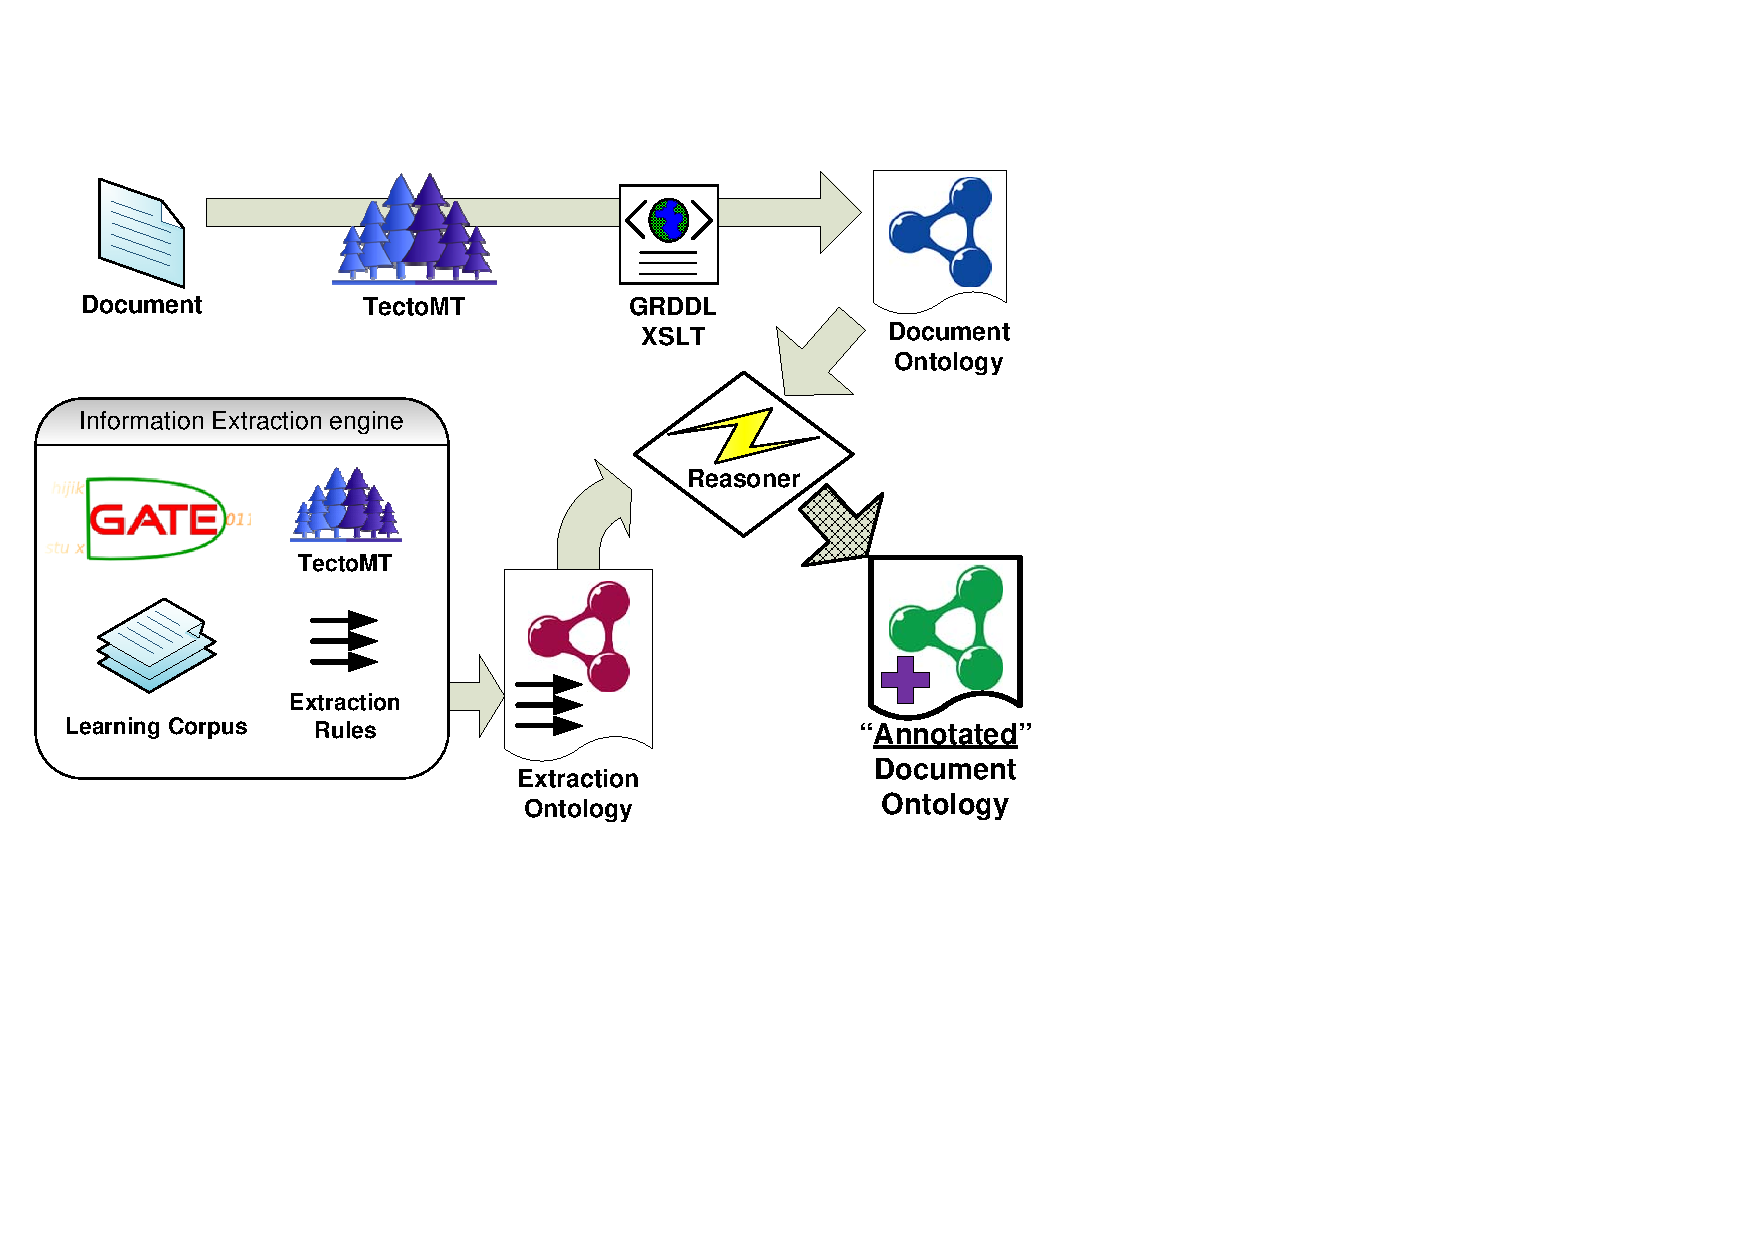
\includegraphics[width=0.6\hsize]{semantic_rules_app_schema}}
\caption{Semantic annotation driven by an extraction ontology and a reasoner -- schema of the process.}
\label{img:rules_app_schema}
\end{figure*}

\clearpage
\subsubsection{Schema of the Case Study}


Schema of the case study can be seen in Fig.~\ref{img:rules_app_schema}.  

The top row of the image illustrates how TectoMT (third party linguistic tool) linguistically annotates an input document and the linguistic annotations are translated to so-called document ontology by a GRDDL/XSLT transformation.

In the bottom of the picture our IE engine learns extraction rules and exports them to an extraction ontology. The reasoner in the middle is used to apply the extraction ontology on the document ontology and it produces the ``annotated'' document ontology, which was described in Section~\ref{sec:doc_ont}.




\subsubsection{How to Download}
All the resources (including source codes of the case study and the experiment) mentioned in this demonstration are publically available on the web-page of our project\footnote{\url{http://czsem.berlios.de/}} and detailed information can be found there.


%%%%%%%%%%%%%%%%%%%%%%%%%%%%%%%%%%%%%%%%%%%%%%%%%%%%%%%%%%%%%%%%%%%%%%%%%%%%%%%%%%%%%%%%%%%%%%%%%%%%%%%%%%%%%%
\section{Experiment} \label{sec:experiment}
%%%%%%%%%%%%%%%%%%%%%%%%%%%%%%%%%%%%%%%%%%%%%%%%%%%%%%%%%%%%%%%%%%%%%%%%%%%%%%%%%%%%%%%%%%%%%%%%%%%%%%%%%%%%%%


In this section we present an experiment that should serve as a proof of a concept that the proposed idea of independent extraction ontologies is working. We have selected several reasoners (namely Jena, HermiT, Pellet and FaCT++) and tested them on two slightly different datasets from two different domains and languages (see Table~\ref{tab:datasets}). This should at least partially demonstrate the universality of the proposed approach.

In both cases the task is to find all instances (corresponding to words in a document) that should be uncovered by the extraction rules. The extraction rules are saved in single extraction ontology for each dataset. The datasets are divided into individual document ontologies (owl files) corresponding to the individual documents. During the experiment the individual document ontologies are processed separately (one ontology in a step) by a selected reasoner. The total time taken to process all document ontologies of a dataset is the measured result of the reasoner for the dataset.

The actual reasoning tasks are more difficult than a simple retrieval of all facts entailed by the extraction rules. Such simple retrieval task took only a few seconds for the Acquisitions v1.1 dataset (including parsing) in the native Prolog environment that the IE engine uses. There were several more inferences needed in the reasoning tasks because the schema of the input files was a little bit different from the schema used in rules. The mapping of the schemas was captured in another ontology that was included in the reasoning. The mapping ontology is a part of the publically available project ontologies\footnote{See ``Data $\rightarrow$ ontologies'' link on the project page \url{http://czsem.berlios.de/}} and a potentially interested reader can find the complete mapping ontology there.


\subsection{Datasets}

In the experiment we used two slightly different datasets from two different domains and languages.  Table~\ref{tab:datasets} summarizes some basic information about them.

\begin{table*}
\centering
\begin{tabular}{|r||r|r|c|r|c|}
\hline
dataset & domain & language & number of files & dataset size & number of rules\\
\hline
\hline
czech\_fireman & accidents & Czech & 50 & 16 MB & 2\\
\hline
acquisitions-v1.1 & finance & English & 600 & 126 MB & 113\\
\hline
\end{tabular}
\caption{Description of datasets that we have used.}
\label{tab:datasets}
\end{table*}


\subsubsection{czech\_fireman}


The fist dataset is called `czech\_fireman'. This dataset was created by ourselves during the development of our IE  engine. It is a collection of 50 Czech texts that are reporting on some accidents (car accidents and other actions of fire rescue services). These reports come from the web of Fire rescue service of Czech Republic\footnote{\url{http://www.hzscr.cz/hasicien/}}. The labeled corpus is publically available on the website of our project\footnote{\url{http://czsem.berlios.de/}}.
The corpus is structured such that each document represents one event (accident) and several attributes of the accident are marked in text. For the experiment we selected the `damage' task -- to find an amount (in CZK - Czech Crowns) of summarized damage arisen during a reported accident.





\subsubsection{Acquisitions v1.1}  

The second dataset is called ``Corporate Acquisition Events'' and it is
described in \cite{lewis1992representation}. More precisely we use the \emph{Acquisitions v1.1} version\footnote{This version of the corpus comes from the Dot.kom (Designing infOrmation extracTion for KnOwledge Management) project's resources: \url{http://nlp.shef.ac.uk/dot.kom/resources.html}} of the corpus.
This is a collection of 600 news articles describing acquisition
events taken from the Reuters dataset. News articles are tagged to identify fields
related to acquisition events. These fields include `purchaser' , `acquired', and
`seller' companies along with their abbreviated names (`purchabr', `acqabr' and
`sellerabr') Some news articles also mention the field `deal amount'.


For the experiment we selected only the `acquired' task.





\subsection{Reasoners}

In the experiment we used four OWL reasoners (namely
Jena\footnote{\url{http://jena.sourceforge.net}}
,HermiT\footnote{\url{http://hermit-reasoner.com}}
,Pellet\footnote{\url{http://clarkparsia.com/pellet}}
and FaCT++\footnote{\url{http://code.google.com/p/factplusplus}}
) and measured the time they needed to process a particular dataset. The time also includes time spend on parsing the input. HermiT, Pellet and FaCT++ were called through OWLAPI-3.1, so the same parser was used for them. Jena reasoner was used in its native environment and used the Jena parser.

In the early beginning of the experiment we had to exclude the FaCT++ reasoner from both tests. It turned out that FaCT++ does not work with rules\footnote{\url{http://en.wikipedia.org/wiki/Semantic_reasoner#Reasoner_comparison}} and it did not return any result instances.  All the remaining reasoners strictly agreed on the results and returned the same sets of instances.

Also HermiT was not fully evaluated on the Acquisitions v1.1 dataset because it was too slow. The reasoner spent 13 hours of running to process only 30 of 600 files of the dataset. And we did not find it useful to let it continue.












\subsection{Evaluation Results of the Experiment}






\begin{table}
\begin{center}
\begin{tabular}{|r||r|r||r|r|}
\hline
reasoner & \textbf{czech\_fireman} & stdev & \textbf{acquisitions-v1.1} & stdev\\
\hline
\hline
Jena & 161 s & 0.226 & 1259 s & 3.579\\
\hline
HermiT & 219 s & 1.636 & $\gg$ 13 hours & \\
\hline
Pellet & 11 s & 0.062 & 503 s & 4.145\\
\hline
FaCT++ & \multicolumn{4}{|c|}{Does not support rules.}\\
\hline
\end{tabular}
\end{center}

Time is measured in seconds. Average values from 6 measurements. Experiment environment: Intel Core I7-920 CPU 2.67GHz, 3GB of RAM, Java SE 1.6.0\_03, Windows XP.

\caption{Time performance of tested reasoners on both datasets.}
\label{tab:results}
\end{table}

Table~\ref{tab:results} summarizes results of the experiment. The standard deviations are relatively small when compared to the differences between the average times.  So there is no doubt about the order of the tested reasoners. Pellet performed the best and HermiT was the slowest amongst the tested and usable reasoners in this experiment.

From the results we can conclude that similar tasks can be satisfactorily solved by contemporary OWL reasoners because three of four tested reasoners were working correctly and two reasoners finished in operational time.






\subsection{Repeatability}

Our implementation is publicly available -- source codes and the datasets can be downloaded from our project's web-page\footnote{\url{http://czsem.berlios.de/}}, so it should be also possible to repeat the experiment in a sense of  the SIGMOD Experimental Repeatability Requirements \cite{biblio:SIGMODrepeatability}.

%%%%%%%%%%%%%%%%%%%%%%%%%%%%%%%%%%%%%%%%%%%%%%%%%%%%%%%%%%%%%%%%%%%%%%%%%%%%%%%%%%%%%%%%%%%%%%%%%%%%%%%%%%%%%%
\section{Future Work}
%%%%%%%%%%%%%%%%%%%%%%%%%%%%%%%%%%%%%%%%%%%%%%%%%%%%%%%%%%%%%%%%%%%%%%%%%%%%%%%%%%%%%%%%%%%%%%%%%%%%%%%%%%%%%%


In this paper (Section~\ref{sec:doc_ont}) we have described a method how to apply an extraction ontology to a document ontology and obtain so called ``annotated'' document ontology. To have an ``annotated'' document ontology is almost the same as to have an annotated document. An annotated document is useful (easier navigation, faster reading and lookup of information, possibility of structured queries on collections of such documents, etc.) but if we are interested in the actual information present in the document, if we want to know the facts that are in a document asserted about the real word things then an annotated document is not sufficient and the conversion of an annotated document to the real world facts is not simple.
There are obvious issues concerning data integration and duplicity of information. For example when in a document two mentions of people are annotated as `injured', what is the number of injured people in the corresponding accident? Are the two annotations in fact linked to the same person or not?

In the beginning of our work on the idea of shareable extraction ontologies we planned to develop it further, we wanted to cover also the step from annotated document ontologies to the real world facts. The extraction process would then end up with so called ``fact ontologies''. But two main obstacles prevent us to do that.

\begin{enumerate}
	\item Our IE engine is not yet capable to solve these data integration and duplicity of information issues. The real world facts would be quite imprecise then.
	\item There are also technology problems of creating new facts (individuals) during reasoning.
\end{enumerate}

Because of the decidability and finality constraints of the Description Logic Reasoning task it is not possible to create new individuals during the reasoning process. There is no standard way how to do it. But there are some proprietary solutions like \verb@swrlx:createOWLThing@\footnote{\url{http://protege.cim3.net/cgi-bin/wiki.pl?action=browse&id=SWRLExtensionsBuiltIns}} from the Prot\'{e}g\'{e} project and \verb@makeTemp(?x)@ or \verb@makeInstance(?x, ?p, ?v)@\footnote{\url{http://jena.sourceforge.net/inference/#RULEbuiltins}} from the Jena project.
And these solutions can be used in the future work. 




%%%%%%%%%%%%%%%%%%%%%%%%%%%%%%%%%%%%%%%%%%%%%%%%%%%%%%%%%%%%%%%%%%%%%%%%%%%%%%%%%%%%%%%%%%%%%%%%%%%%%%%%%%%%%%
\section{Conclusion -- the Main Contributions}
%%%%%%%%%%%%%%%%%%%%%%%%%%%%%%%%%%%%%%%%%%%%%%%%%%%%%%%%%%%%%%%%%%%%%%%%%%%%%%%%%%%%%%%%%%%%%%%%%%%%%%%%%%%%%%

In the end of the paper we would like to summarize the main contributions of the paper.

\begin{itemize}
	\item In the beginning of the paper we pointed out the draw back of so called extraction ontologies -- in most cases they are dependent on a particular extraction/annotation tool and they cannot be used separately.	
	\item We extended the concept of extraction ontologies by adding the shareable aspect and we introduced a new principle of making extraction ontologies independent of the original tool: the possibility of application of an extraction ontology to a document by an ordinary reasoner.
	\item In Section~\ref{sec:case} we presented a case study that shows that the idea of shareable extraction ontologies is realizable. We presented implementation of an IE tool that exports its extraction rules to an extraction ontology and we demonstrated how this extraction ontology can be applied to a document by a reasoner.
	\item Moreover in Section~\ref{sec:experiment} an experiment with several OWL reasoners was presented. The experiment evaluated the performance of contemporary OWL reasoners on IE tasks: application of extraction ontologies.  
	\item A new publically available benchmark for OWL reasoning was created together with the experiment. Other reasoners can be tested this way.
\end{itemize}
   

We would like to conclude the paper by stating that even if the fundamental idea of the paper will not set up in the community it is at least a new use case for both: usage of IE tools and reasoners.























% An example of a floating figure using the graphicx package.
% Note that \label must occur AFTER (or within) \caption.
% For figures, \caption should occur after the \includegraphics.
% Note that IEEEtran v1.7 and later has special internal code that
% is designed to preserve the operation of \label within \caption
% even when the captionsoff option is in effect. However, because
% of issues like this, it may be the safest practice to put all your
% \label just after \caption rather than within \caption{}.
%
% Reminder: the "draftcls" or "draftclsnofoot", not "draft", class
% option should be used if it is desired that the figures are to be
% displayed while in draft mode.
%
%\begin{figure}[!t]
%\centering
%\includegraphics[width=2.5in]{myfigure}
% where an .eps filename suffix will be assumed under latex, 
% and a .pdf suffix will be assumed for pdflatex; or what has been declared
% via \DeclareGraphicsExtensions.
%\caption{Simulation Results}
%\label{fig_sim}
%\end{figure}

% Note that IEEE typically puts floats only at the top, even when this
% results in a large percentage of a column being occupied by floats.


% An example of a double column floating figure using two subfigures.
% (The subfig.sty package must be loaded for this to work.)
% The subfigure \label commands are set within each subfloat command, the
% \label for the overall figure must come after \caption.
% \hfil must be used as a separator to get equal spacing.
% The subfigure.sty package works much the same way, except \subfigure is
% used instead of \subfloat.
%
%\begin{figure*}[!t]
%\centerline{\subfloat[Case I]\includegraphics[width=2.5in]{subfigcase1}%
%\label{fig_first_case}}
%\hfil
%\subfloat[Case II]{\includegraphics[width=2.5in]{subfigcase2}%
%\label{fig_second_case}}}
%\caption{Simulation results}
%\label{fig_sim}
%\end{figure*}
%
% Note that often IEEE papers with subfigures do not employ subfigure
% captions (using the optional argument to \subfloat), but instead will
% reference/describe all of them (a), (b), etc., within the main caption.


% An example of a floating table. Note that, for IEEE style tables, the 
% \caption command should come BEFORE the table. Table text will default to
% \footnotesize as IEEE normally uses this smaller font for tables.
% The \label must come after \caption as always.
%
%\begin{table}[!t]
%% increase table row spacing, adjust to taste
%\renewcommand{\arraystretch}{1.3}
% if using array.sty, it might be a good idea to tweak the value of
% \extrarowheight as needed to properly center the text within the cells
%\caption{An Example of a Table}
%\label{table_example}
%\centering
%% Some packages, such as MDW tools, offer better commands for making tables
%% than the plain LaTeX2e tabular which is used here.
%\begin{tabular}{|c||c|}
%\hline
%One & Two\\
%\hline
%Three & Four\\
%\hline
%\end{tabular}
%\end{table}


% Note that IEEE does not put floats in the very first column - or typically
% anywhere on the first page for that matter. Also, in-text middle ("here")
% positioning is not used. Most IEEE journals/conferences use top floats
% exclusively. Note that, LaTeX2e, unlike IEEE journals/conferences, places
% footnotes above bottom floats. This can be corrected via the \fnbelowfloat
% command of the stfloats package.




% use section* for acknowledgement
\section*{Acknowledgment}
This work was partially supported by Czech projects: GACR P202/10/0761, GACR-201/09/H057, GAUK 31009 and MSM-0021620838.




% trigger a \newpage just before the given reference
% number - used to balance the columns on the last page
% adjust value as needed - may need to be readjusted if
% the document is modified later
%\IEEEtriggeratref{8}
% The "triggered" command can be changed if desired:
%\IEEEtriggercmd{\enlargethispage{-5in}}

% references section

% can use a bibliography generated by BibTeX as a .bbl file
% BibTeX documentation can be easily obtained at:
% http://www.ctan.org/tex-archive/biblio/bibtex/contrib/doc/
% The IEEEtran BibTeX style support page is at:
% http://www.michaelshell.org/tex/ieeetran/bibtex/
\bibliographystyle{IEEEtran}
% argument is your BibTeX string definitions and bibliography database(s)

\bibliography{DedekVojtas_WI_IAT2011_semantically}
%
% <OR> manually copy in the resultant .bbl file
% set second argument of \begin to the number of references
% (used to reserve space for the reference number labels box)
%\begin{thebibliography}{1}
%
%\bibitem{IEEEhowto:kopka}
%H.~Kopka and P.~W. Daly, \emph{A Guide to \LaTeX}, 3rd~ed.\hskip 1em plus
%  0.5em minus 0.4em\relax Harlow, England: Addison-Wesley, 1999.
%
%\end{thebibliography}




% that's all folks
\end{document}


